\documentclass[11pt]{article}
\usepackage[margin=1in]{geometry}
\usepackage{amsmath}
\usepackage{booktabs}
\usepackage{graphicx}
\usepackage{hyperref}

\title{HW1 Writeup: Linear and Neural Sentiment Classification}
\author{Zhizhe Zhang}
\date{}

\begin{document}
\maketitle

\section{Implementation Summary}
I implemented all required components in \texttt{models.py}:
\begin{itemize}
    \item \texttt{UnigramFeatureExtractor}, \texttt{BigramFeatureExtractor}, \texttt{BetterFeatureExtractor}
    \item \texttt{LogisticRegressionClassifier} and \texttt{train\_logistic\_regression}
    \item \texttt{NeuralSentimentClassifier}, \texttt{DANNetwork}, and \texttt{train\_deep\_averaging\_network}
\end{itemize}

For logistic regression, I used sparse bag-of-words features with SGD, random shuffling each epoch, a decayed learning-rate schedule
\[
\eta_t = \frac{\eta_0}{1 + 0.05 \cdot \text{epoch}},
\]
and a small L2 shrinkage term.

For DAN, each sentence is converted to word indices, embeddings are averaged, and a feed-forward network
(\texttt{Linear $\to$ ReLU $\to$ Dropout $\to$ Linear}) predicts two classes. Training uses Adam + NLLLoss, and I keep the best dev checkpoint.

\section{Required Results}
\begin{table}[h]
\centering
\begin{tabular}{lccc}
\toprule
Command & Dev Accuracy & Dev F1 & Time \\
\midrule
\texttt{python sentiment\_classifier.py --model LR --feats UNIGRAM} & 0.7718 & 0.7858 & 1.47s \\
\texttt{python sentiment\_classifier.py --model DAN} & 0.7970 & 0.8066 & 16.60s \\
\bottomrule
\end{tabular}
\caption{Main required results. Both models exceed the 77\% dev accuracy threshold.}
\end{table}

\section{Exploration 1: LR Learning-Rate Schedules}
I compared two initial step sizes (\texttt{--lr 0.05} and \texttt{--lr 0.2}) for UNIGRAM LR with 25 epochs and tracked:
\begin{itemize}
    \item average training log-likelihood per epoch
    \item dev accuracy per epoch
\end{itemize}

Final dev accuracies:
\begin{itemize}
    \item \texttt{--lr 0.05}: dev acc = 0.7695
    \item \texttt{--lr 0.2}: dev acc = 0.7729
\end{itemize}

Figure~\ref{fig:lr-curves} shows that larger learning rate improves the training objective faster, but dev accuracy remains very close between the two settings.

\begin{figure}[h]
\centering
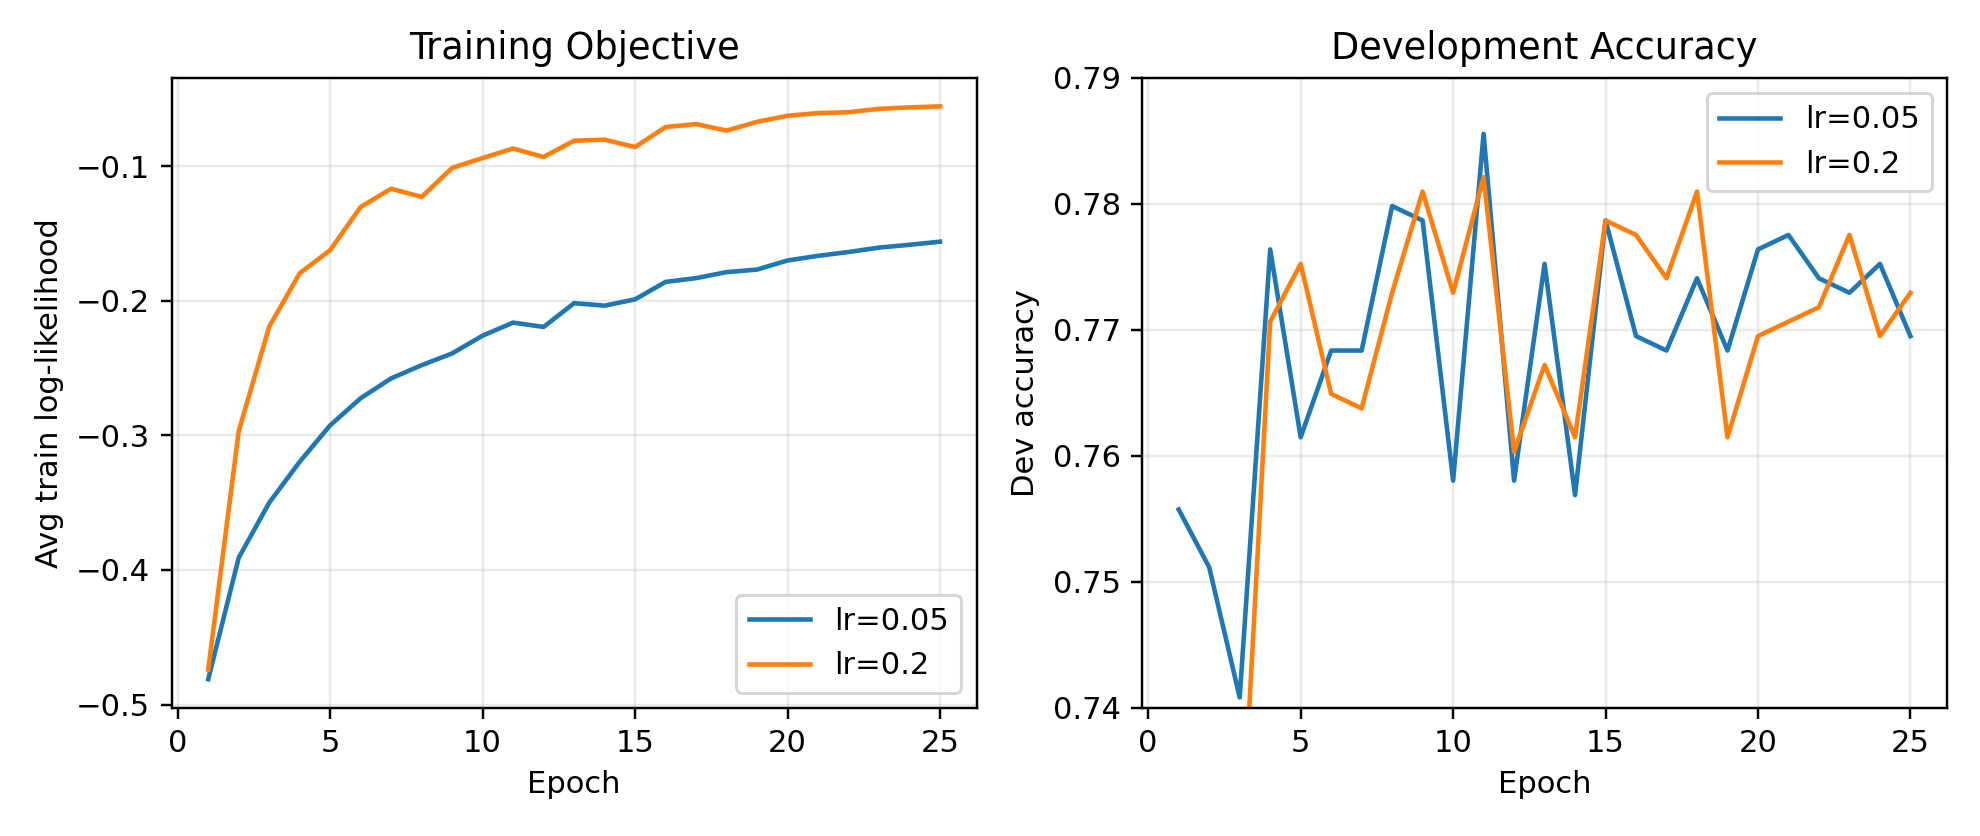
\includegraphics[width=\linewidth]{lr_schedule_curves.png}
\caption{Training objective and dev accuracy versus epoch for two LR schedules.}
\label{fig:lr-curves}
\end{figure}

\section{Exploration 2: Feature Modifications}
With \texttt{--lr 0.1 --num\_epochs 25}:
\begin{itemize}
    \item \texttt{--feats BIGRAM}: dev acc = 0.7351
    \item \texttt{--feats BETTER}: dev acc = 0.8085
\end{itemize}

My \texttt{BETTER} extractor is not a unigram+bigram concatenation. It uses:
\begin{itemize}
    \item stopword filtering and short-token filtering
    \item clipped unigram counts (\texttt{1/2} instead of raw counts)
    \item negation scope marking (next 3 content words get \texttt{\_NEG})
    \item a sentence-level intensifier indicator feature
\end{itemize}

Observation: BIGRAM overfits strongly, while these modified features improve dev performance.

\section{Additional DAN Check}
I also compared DAN variants:
\begin{itemize}
    \item 50d embeddings: dev acc = 0.7431
    \item 300d embeddings + hidden size 200: dev acc = 0.7936
\end{itemize}

This suggests that embedding dimensionality (300d vs 50d) has a strong effect, while increasing hidden size alone does not reliably beat the baseline.

\end{document}
